\documentclass[10pt,landscape,a4paper]{article}
\usepackage{nonfloat}
\usepackage{multicol}
\usepackage[font=scriptsize]{caption}
\usepackage{calc}
\usepackage{ifthen}
\usepackage[landscape]{geometry}
\usepackage{amsmath}
\usepackage{amssymb}
\usepackage{multirow}

\usepackage{graphics}
   \usepackage[pdftex]{graphicx}
\usepackage{epstopdf}
 \usepackage{ifpdf}
\usepackage{sectsty}
\paragraphfont{\small}

% To make this come out properly in landscape mode, do one of the following
% 1.
%  pdflatex latexsheet.tex
%
% 2.
%  latex latexsheet.tex
%  dvips -P pdf  -t landscape latexsheet.dvi
%  ps2pdf latexsheet.ps


% If you're reading this, be prepared for confusion.  Making this was
% a learning experience for me, and it shows.  Much of the placement
% was hacked in; if you make it better, let me know...


% 2008-04
% Changed page margin code to use the geometry package. Also added code for
% conditional page margins, depending on paper size. Thanks to Uwe Ziegenhagen
% for the suggestions.

% 2006-08
% Made changes based on suggestions from Gene Cooperman. <gene at ccs.neu.edu>


% To Do:
% \listoffigures \listoftables
% \setcounter{secnumdepth}{0}


% This sets page margins to .5 inch if using letter paper, and to 1cm
% if using A4 paper. (This probably isn't strictly necessary.)
% If using another size paper, use default 1cm margins.
\ifthenelse{\lengthtest { \paperwidth = 11in}}
	{ \geometry{top=.5in,left=.5in,right=.5in,bottom=.5in} }
	{\ifthenelse{ \lengthtest{ \paperwidth = 297mm}}
		{\geometry{top=1cm,left=1cm,right=1cm,bottom=1cm} }
		{\geometry{top=1cm,left=1cm,right=1cm,bottom=1cm} }
	}

% Turn off header and footer
\pagestyle{empty}
 

% Redefine section commands to use less space
\makeatletter
\renewcommand{\section}{\@startsection{section}{1}{0mm}%
                                {-1ex plus -.5ex minus -.2ex}%
                                {0.5ex plus .2ex}%x
                                {\normalfont\large\bfseries}}
\renewcommand{\subsection}{\@startsection{subsection}{2}{0mm}%
                                {-1explus -.5ex minus -.2ex}%
                                {0.5ex plus .2ex}%
                                {\normalfont\normalsize\bfseries}}
\renewcommand{\subsubsection}{\@startsection{subsubsection}{3}{0mm}%
                                {-1ex plus -.5ex minus -.2ex}%
                                {1ex plus .2ex}%
                                {\normalfont\small\bfseries}}
\makeatother

% Define BibTeX command
\def\BibTeX{{\rm B\kern-.05em{\sc i\kern-.025em b}\kern-.08em
    T\kern-.1667em\lower.7ex\hbox{E}\kern-.125emX}}

% Don't print section numbers
\setcounter{secnumdepth}{0}


\setlength{\parindent}{0pt}
\setlength{\parskip}{0pt plus 0.5ex}

 % figures
\newcommand{\sizes}{3.4} % selbstdefinierte Punktgrösse in Bilder
\newcommand{\sizem}{5.1}% selbstdefinierte Punktgrösse in Bilder

%math
\newcommand{\dd}{\textnormal{d}}
\newcommand{\dt}{\textnormal{d}t}
\newcommand{\DD}{\textnormal{D}}
\newcommand{\Dt}{\textnormal{D}t}
\newcommand{\deta}{\textnormal{d}\eta}
\newcommand{\argmin}{\mathop{\mathrm{argmin}}}
\newcommand{\Upr}{{\mathop{\mathrm{Upr}}}}
\newcommand{\Sgn}{{\mathop{\mathrm{Sgn}}}}
\newcommand{\h}{\mathop{\mathrm{H}}}
\newcommand{\prox}{{\mathop{\mathrm{prox}}}}
\newcommand{\abs}{\mathop{\mathrm{abs}}}
\newcommand{\T}{^{\mathop{\mathrm{T}}}}
\newcommand{\diag}{{\mathop{\mathrm{diag}}}}


%boldmath
%bold operator
\newcommand{\vna}{\mbox{\boldmath $\nabla$}}
%bold greek
\newcommand{\val}{\mbox{\boldmath $\alpha$}}
\newcommand{\vbe}{\mbox{\boldmath $\beta$}}
\newcommand{\vga}{\mbox{\boldmath $\gamma$}}
\newcommand{\vde}{\mbox{\boldmath $\delta$}}
\newcommand{\vep}{\mbox{\boldmath $\epsilon$}}
\newcommand{\vze}{\mbox{\boldmath $\zeta$}}
\newcommand{\vet}{\mbox{\boldmath $\eta$}}
\newcommand{\vth}{\mbox{\boldmath $\theta$}}
\newcommand{\vio}{\mbox{\boldmath $\iota$}}
\newcommand{\vka}{\mbox{\boldmath $\kappa$}}
\newcommand{\vla}{\mbox{\boldmath $\lambda$}}
\newcommand{\vmu}{\mbox{\boldmath $\mu$}}
\newcommand{\vnu}{\mbox{\boldmath $\nu$}}
\newcommand{\vxi}{\mbox{\boldmath $\xi$}}
\newcommand{\vpi}{\mbox{\boldmath $\pi$}}
\newcommand{\vrh}{\mbox{\boldmath $\rho$}}
\newcommand{\vsi}{\mbox{\boldmath $\sigma$}}
\newcommand{\vta}{\mbox{\boldmath $\tau$}}
\newcommand{\vup}{\mbox{\boldmath $\upsilon$}}
\newcommand{\vph}{\mbox{\boldmath $\varphi$}}
\newcommand{\vch}{\mbox{\boldmath $\chi$}}
\newcommand{\vps}{\mbox{\boldmath $\psi$}}
\newcommand{\vom}{\mbox{\boldmath $\omega$}}

\newcommand{\vvep}{\mbox{\boldmath $\varepsilon$}}
\newcommand{\vvth}{\mbox{\boldmath $\vartheta$}}
\newcommand{\vvrh}{\mbox{\boldmath $\varrho$}}
\newcommand{\vvpi}{\mbox{\boldmath $\varpi$}}
\newcommand{\vvsi}{\mbox{\boldmath $\varsigma$}}
\newcommand{\vvph}{\mbox{\boldmath $\phi$}}

%bold capital greek
\newcommand{\vGa}{\mathbf \Gamma}
\newcommand{\vDe}{\mathbf \Delta}
\newcommand{\vTh}{\mathbf \Theta}
\newcommand{\vLa}{\mathbf \Lambda}
\newcommand{\vXi}{\mathbf \Xi}
\newcommand{\vPi}{\mathbf \Pi}
\newcommand{\vSi}{\mathbf \Sigma}
\newcommand{\vUp}{\mathbf \Upsilon}
\newcommand{\vPh}{\mathbf \Phi}
\newcommand{\vPs}{\mathbf \Psi}
\newcommand{\vOm}{\mathbf \Omega}

%capital greek slanted, OHNE amsmath-package
%\newcommand{\iGa}{\mathnormal{\Gamma}}
%\newcommand{\iDe}{\mathnormal{\Delta}}
%\newcommand{\iTh}{\mathnormal{\Theta}}
%\newcommand{\iLa}{\mathnormal{\Lambda}}
%\newcommand{\iXi}{\mathnormal{\Xi}}
%\newcommand{\iPi}{\mathnormal{\Pi}}
%\newcommand{\iSi}{\mathnormal{\Sigma}}
%\newcommand{\iUp}{\mathnormal{\Upsilon}}
%\newcommand{\iPh}{\mathnormal{\Phi}}
%\newcommand{\iPs}{\mathnormal{\Psi}}
%\newcommand{\iOm}{\mathnormal{\Omega}}

%capital greek slanted, MIT amsmath-package
\newcommand{\iGa}{\varGamma}
\newcommand{\iDe}{\varDelta}
\newcommand{\iTh}{\varTheta}
\newcommand{\iLa}{\varLambda}
\newcommand{\iXi}{\varXi}
\newcommand{\iPi}{\varPi}
\newcommand{\iSi}{\varSigma}
\newcommand{\iUp}{\varUpsilon}
\newcommand{\iPh}{\varPhi}
\newcommand{\iPs}{\varPsi}
\newcommand{\iOm}{\varOmega}

%bold latin
\newcommand{\va}{\mathbf a}
\newcommand{\vb}{\mathbf b}
\newcommand{\vc}{\mathbf c}
\newcommand{\vd}{\mathbf d}
\newcommand{\ve}{\mathbf e}
\newcommand{\vf}{\mathbf f}
\newcommand{\vg}{\mathbf g}
\newcommand{\vh}{\mathbf h}
\newcommand{\vi}{\mathbf i}
\newcommand{\vj}{\mathbf j}
\newcommand{\vk}{\mathbf k}
\newcommand{\vl}{\mathbf l}
\newcommand{\vm}{\mathbf m}
\newcommand{\vn}{\mathbf n}
\newcommand{\vo}{\mathbf o}
\newcommand{\vp}{\mathbf p}
\newcommand{\vq}{\mathbf q}
\newcommand{\vr}{\mathbf r}
\newcommand{\vs}{\mathbf s}
\newcommand{\vt}{\mathbf t}
\newcommand{\vu}{\mathbf u}
\newcommand{\vv}{\mathbf v}
\newcommand{\vw}{\mathbf w}
\newcommand{\vx}{\mathbf x}
\newcommand{\vy}{\mathbf y}
\newcommand{\vz}{\mathbf z}
\newcommand{\eins}{\mathbf 1}

%bold capital latin
\newcommand{\vA}{\mathbf A}
\newcommand{\vB}{\mathbf B}
\newcommand{\vC}{\mathbf C}
\newcommand{\vD}{\mathbf D}
\newcommand{\vE}{\mathbf E}
\newcommand{\vF}{\mathbf F}
\newcommand{\vG}{\mathbf G}
\newcommand{\vH}{\mathbf H}
\newcommand{\vI}{\mathbf I}
\newcommand{\vJ}{\mathbf J}
\newcommand{\vK}{\mathbf K}
\newcommand{\vL}{\mathbf L}
\newcommand{\vM}{\mathbf M}
\newcommand{\vN}{\mathbf N}
\newcommand{\vO}{\mathbf O}
\newcommand{\vP}{\mathbf P}
\newcommand{\vQ}{\mathbf Q}
\newcommand{\vR}{\mathbf R}
\newcommand{\vS}{\mathbf S}
\newcommand{\vT}{\mathbf T}
\newcommand{\vU}{\mathbf U}
\newcommand{\vV}{\mathbf V}
\newcommand{\vW}{\mathbf W}
\newcommand{\vX}{\mathbf X}
\newcommand{\vY}{\mathbf Y}
\newcommand{\vZ}{\mathbf Z}

%calligraphic
\newcommand{\cA}{\mathcal{A}}
\newcommand{\cB}{\mathcal{B}}
\newcommand{\cC}{\mathcal{C}}
\newcommand{\cD}{\mathcal{D}}
\newcommand{\cE}{\mathcal{E}}
\newcommand{\cF}{\mathcal{F}}
\newcommand{\cG}{\mathcal{G}}
\newcommand{\cH}{\mathcal{H}}
\newcommand{\cI}{\mathcal{I}}
\newcommand{\cJ}{\mathcal{J}}
\newcommand{\cK}{\mathcal{K}}
\newcommand{\cL}{\mathcal{L}}
\newcommand{\cM}{\mathcal{M}}
\newcommand{\cN}{\mathcal{N}}
\newcommand{\cO}{\mathcal{O}}
\newcommand{\cP}{\mathcal{P}}
\newcommand{\cQ}{\mathcal{Q}}
\newcommand{\cR}{\mathcal{R}}
\newcommand{\cS}{\mathcal{S}}
\newcommand{\cT}{\mathcal{T}}
\newcommand{\cU}{\mathcal{U}}
\newcommand{\cV}{\mathcal{V}}
\newcommand{\cW}{\mathcal{W}}
\newcommand{\cX}{\mathcal{X}}
\newcommand{\cY}{\mathcal{Y}}
\newcommand{\cZ}{\mathcal{Z}}

%fraktur
\newcommand{\frA}{\mathfrak{A}}
\newcommand{\frB}{\mathfrak{B}}
\newcommand{\frC}{\mathfrak{C}}
\newcommand{\frD}{\mathfrak{D}}
\newcommand{\frE}{\mathfrak{E}}
\newcommand{\frF}{\mathfrak{F}}
\newcommand{\frG}{\mathfrak{G}}
\newcommand{\frH}{\mathfrak{H}}
\newcommand{\frI}{\mathfrak{I}}
\newcommand{\frJ}{\mathfrak{J}}
\newcommand{\frK}{\mathfrak{K}}
\newcommand{\frL}{\mathfrak{L}}
\newcommand{\frM}{\mathfrak{M}}
\newcommand{\frN}{\mathfrak{N}}
\newcommand{\frO}{\mathfrak{O}}
\newcommand{\frP}{\mathfrak{P}}
\newcommand{\frQ}{\mathfrak{Q}}
\newcommand{\frR}{\mathfrak{R}}
\newcommand{\frS}{\mathfrak{S}}
\newcommand{\frT}{\mathfrak{T}}
\newcommand{\frU}{\mathfrak{U}}
\newcommand{\frV}{\mathfrak{V}}
\newcommand{\frW}{\mathfrak{W}}
\newcommand{\frX}{\mathfrak{X}}
\newcommand{\frY}{\mathfrak{Y}}
\newcommand{\frZ}{\mathfrak{Z}}

\newcommand{\fra}{\mathfrak{a}}
\newcommand{\frb}{\mathfrak{b}}
\newcommand{\frc}{\mathfrak{c}}
\newcommand{\frd}{\mathfrak{d}}
\newcommand{\fre}{\mathfrak{e}}
\newcommand{\frf}{\mathfrak{f}}
\newcommand{\frg}{\mathfrak{g}}
\newcommand{\frh}{\mathfrak{h}}
\newcommand{\fri}{\mathfrak{i}}
\newcommand{\frj}{\mathfrak{j}}
\newcommand{\frk}{\mathfrak{k}}
\newcommand{\frl}{\mathfrak{l}}
\newcommand{\frm}{\mathfrak{m}}
\newcommand{\frn}{\mathfrak{n}}
\newcommand{\fro}{\mathfrak{o}}
\newcommand{\frp}{\mathfrak{p}}
\newcommand{\frq}{\mathfrak{q}}
\newcommand{\frr}{\mathfrak{r}}
\newcommand{\frs}{\mathfrak{s}}
\newcommand{\frt}{\mathfrak{t}}
\newcommand{\fru}{\mathfrak{u}}
\newcommand{\frv}{\mathfrak{v}}
\newcommand{\frw}{\mathfrak{w}}
\newcommand{\frx}{\mathfrak{x}}
\newcommand{\fry}{\mathfrak{y}}
\newcommand{\frz}{\mathfrak{z}}

% -----------------------------------------------------------------------
\DeclareGraphicsExtensions{.pdf,.eps}
 \DeclareMathOperator{\tr}{tr}



\newcommand\myfigure[1]{%
\medskip\noindent\begin{minipage}{\columnwidth}
\centering%
#1%
%figure,caption, and label go here
\end{minipage}\medskip}

\begin{document}

\raggedright
\footnotesize
\begin{multicols}{2}


% multicol parameters
% These lengths are set only within the two main columns
%\setlength{\columnseprule}{0.25pt}
\setlength{\premulticols}{1pt}
\setlength{\postmulticols}{1pt}
\setlength{\multicolsep}{1pt}
\setlength{\columnsep}{2pt}

\begin{center}
     \Large{\textbf{Robot Math Cheat Sheet}} \\
\end{center}
%%%%%%%%%%%%%%%%%%%%%%%%%%%%%%%%%%%%%%%%%%%%%%%%%%%%%%%%%%%%%%%%%%%%%%%%%%%%%%%%%%%%%%%
%  BEGIN CONTENT
%%%%%%%%%%%%%%%%%%%%%%%%%%%%%%%%%%%%%%%%%%%%%%%%%%%%%%%%%%%%%%%%%%%%%%%%%%%%%%%%%%%%%%%
\section{Nomenclature }
\begin{tabular}{|l|l|l|}
\hline
Coordinate system (CS) & ${\ve_x^B,\ve_y^B,\ve_z^B}$ & Cartesian right-hand system $B$ with basis (unit) vectors $\ve$  \\ \hline
Position vector & ${}_I\vr_{OP} \in \mathbb{R}^3 $ & vector from point $O$ to point $P$ expressed in CS $I$ \\ \hline 
Translational velocity & ${}_I\vv_P \in \mathbb{R}^3 $  & translational velocity of point $P$ expressed in CS $I$ \\ \hline
Angular velocity & ${}_I\vom_{IB} \in \mathbb{R}^3 $ & ang. velocity of CS $B$ w.r.t. to CS $B$ expressed in CS $I$ \\ \hline
Ang. vel. of rigid body & ${}_B\vOm = {}_B\vom_{IB}$ & with body-fixed CS $B$ and inertial CS $I$ \\ \hline
Ang. acc. of rigid body & ${}_B\vPs$ \\ \hline
% Generalized coordinates & $\vq \in \mathbb{Q} \subset \mathbb{R}^{n_q}$ & set of coordinates to describe a multi-rigid-body system\\ \hline
% Generalized velocities & $\vu \in \mathbb{U} \subset \mathbb{R}^{n_u}$ & gen. velocities of multi-rigid-body system, where $\vu = \vF\dot{\vq}$\\ \hline
Cross product & \multicolumn{2}{l|}{$\va \times \vb = \begin{pmatrix} a_1 \\ a_2 \\ a_3\end{pmatrix} \times \begin{pmatrix} b_1 \\ b_2 \\ b_3\end{pmatrix} =  \tilde{\va}\vb = \begin{pmatrix} 0 & -a_3 & a_2 \\ a_3 & 0 & -a_1 \\ -a_2 & a_1 & 0 \end{pmatrix} \begin{pmatrix} b_1 \\ b_2 \\ b_3\end{pmatrix}$}  \\ \hline
Euclidean norm & \multicolumn{2}{l|}{$\lVert \va \rVert = \sqrt{\va^T\va} = \sqrt{a_1^2 + a_2^2 + a_3^2}$} \\ \hline
Machine precision & $\epsilon$ & \\ \hline
\end{tabular}

\section{Coordinate Transformations and Rotations}
\begin{tabular}{|l|l@{}|l@{}|}
\hline
Rotation  & $\vR_{BI} \in \mathrm{SO}(3)$ & The 3D rotation $\vR_{BI}:\cI \rightarrow \cB$ rotates a vector \\ 
matrix & ${}_I\vR_{BI} = ({}_I\ve_x^B, {}_I\ve_y^B, {}_I\ve_z^B)$ & by mapping it from $\cI$ to $\cB$. \\
& & The transformation is active (alibi).\\ \hline
Basis-& $\vA_{BI} = \vA_{I}^{B}\in \mathrm{SO}(3)$ & Transforms the coord. of a vector expr. in CS $I$ to CS $B$,\\  
Transformation  & ${}_{B}\vr_{OP} = \vA_{BI} {}_{I}\vr_{OP}$ &  i.e.\ the coord. of a point $P$ change due to a rotation of \\
matrix& &  the CS and the vector $\vr_{OP}$ representing $P$ is not rotated. \\  
 & $\vA_{BI} = \vA_{IB}^T = {}_I \vR_{BI}^T$ & The transformation is passive (alias).\\ \hline
 Unit  & $\vp_{BI}=(a_0, \va)\in \mathbb{H}$ &  Rotates a vector by mapping it from $\cI$ to $\cB$ (active, alibi). \\
Quaternion& $\va = (a_1, a_2 ,a_3)^T$  & The transformation is active (alibi). \\ 
 & $\left\lVert\vp_{BI}\right\rVert=1$  &   \\ \hline
Angle-axis & $\{\chi, \vn\}_{BI}, \chi \in [-\frac{\pi}{2}, \frac{\pi}{2})$ & Rotates a vector by mapping it from $\cI$ to $\cB$  (active, alibi) \\
& $\lVert\vn\rVert=1$ & with angle $\chi$ around unit vector \\ \hline
Yaw-pitch-roll &  $(\psi, \theta, \phi)_{BI}^T$  & Tait-Bryan angles: $z-y'-x''$ (Singularity: $\theta=\pm\frac{\pi}{2}$) \\
 (Flight conv.) & $\cI \rightarrow \cB$ & $\psi\in(-\pi,\pi), \theta\in(-\frac{\pi}{2},\frac{\pi}{2}), \phi\in(-\pi,\pi)$  \\  \hline
Roll-pitch-yaw &  $(\alpha, \beta, \gamma)_{BI}^T$ & Cardan angles: $x-y'-z''$ (Singularity: $\beta=\pm\frac{\pi}{2}$)  \\
 (Glocker conv.)& $\cI \rightarrow \cB$ & $\alpha\in(-\pi,\pi), \beta\in(-\frac{\pi}{2},\frac{\pi}{2}), \gamma\in(-\pi,\pi)$  \\  \hline
\end{tabular} % \multirow{2}{*}{}
\subsection{Unit Quaternions}
Hamiltonian convention: 
$\boxed{\begin{aligned}\vp_{BI} &= a_0 + a_1 i + a_2 j + a_3 k \in \mathbb{H}, \quad a_i \in \mathbb{R}  \\
i^2 &= j^2=k^2 = ijk = -1 \\
\| \vp_{BI} \| &= \sqrt{a_0^2 + \va^T\va} = 1
\end{aligned}}$  \\

Inverse of quaternion: $\vp_{IB} = \vp_{BI}^{-1} = \bar{\vp}_{BI} = (a_0, -\va)$ \\
Quaternion as a vector: $\Psi: \mathbb{H} \rightarrow \mathbb{R}^4, \Psi\left ( (a_0, \va) \right) = \begin{pmatrix} a_0 \\ \va \end{pmatrix}$ \\
Quaternion multiplication: $\begin{aligned}\vp_{CA} &= \vp_{CB} \cdot \vp_{BA} = (a_0, \va)\cdot(b_0, \vb) = (a_0 b_0 - \va^{T} \vb, a_{0} \vb + b_0 \va + \tilde{\va} \vb)  \\
	  &\Leftrightarrow \vQ\left((a_0, \va)\right)\Psi\left((b_0, \vb)\right) = \begin{pmatrix}a_0 & -\va^T \\  \va & a_0\vI_{3x3}+\tilde{\va} \\ \end{pmatrix} \begin{pmatrix} b_0 \\ b_1 \\ b_2 \\ b_3 \end{pmatrix} 
	  = \begin{pmatrix} 
 a_0 & -a_1 & -a_2 & -a_3 \\
 a_1 &  a_0 & -a_3 &  a_2 \\
 a_2 &  a_3 &  a_0 & -a_1 \\
 a_3 & -a_2 &  a_1 &  a_0 \\ \end{pmatrix}\begin{pmatrix} b_0 \\ b_1 \\ b_2 \\ b_3 \end{pmatrix}  \\
 &= \vQ\left((b_0, \vb)\right)^T\Psi\left((a_0, \va)\right) \\
\end{aligned}$ \\
$\vp_{BI}$ and $-\vp_{BI}$ yield the same rotation. \\
\subsection{Yaw-Pitch-Roll $\Leftrightarrow$ Rotation Matrix}
\myfigure{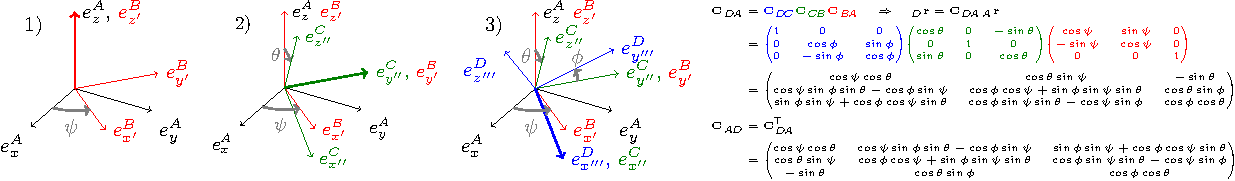
\includegraphics[width=1\columnwidth]{coordinate_systems/coordinate_system_ypr-crop.pdf}\vspace{-3mm}
\figcaption{Rotation from $I$-frame to $B$-frame: ($z-y'-x''$) -- (yaw-pitch-roll) -- ($\psi-\theta-\phi$) -- ($50^\circ-25^\circ-30^\circ)$}\label{fig:yaw-pitch-roll}}
\subsection{Roll-Pitch-Yaw $\Leftrightarrow$ Rotation Matrix}
\myfigure{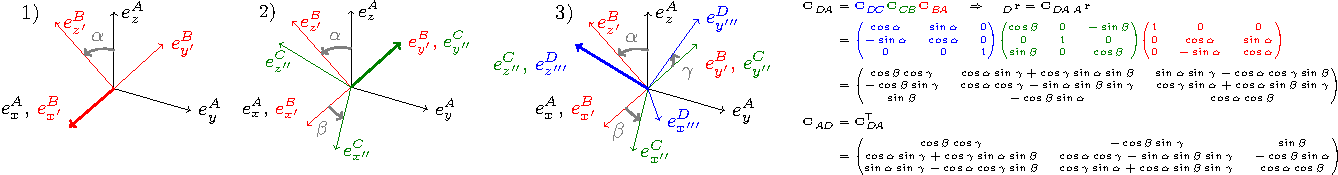
\includegraphics[width=1\columnwidth]{coordinate_systems/coordinate_system_rpy-crop.pdf}\vspace{-3mm}
\figcaption{Rotation from $I$-frame to $B$-frame: ($x-y'-z''$) -- (roll-pitch-yaw) -- ($\alpha-\beta-\gamma$) -- ($50^\circ-25^\circ-30^\circ)$}\label{fig:roll-pitch-yaw}}

\subsection{Successive Composition of Rotations}
$\vp_{IB} = \vp_{ID} \vp_{DC} \vp_{CB} \Leftrightarrow \vA_{BI} = \vA_{BC}\vA_{CD}\vA_{DI}$

\subsection{Transformation of a Vector}

${}_{B}\vr_{OP} = \vA_{BI} {}_{I}\vr_{OP}$

$(0, {}_B\vr_{OP}) = \vp_{IB} (0, {}_I\vr_{OP}) \vp_{IB}^{-1}$ ????



%$\begin{aligned}{}_B\vr_{OP} &= {}_I\vr_{OP} + 2a_0\tilde{\va} {}_I\vr_{OP} + 2 \tilde{\va}^2 {}_I\vr_{OP}, \quad  \text{(Eigen)} \\
% &= \vp_{BI} (0, {}_I\vr_{OP}^T)^T \vp_{BI}^{-1} = (a_0, \va^T)^T (0, {}_I\vr_{OP}^T)^T (a_0, -\va^T)^T \end{aligned}$



\subsection{Quaternion $\Leftrightarrow$ Angle-Axis}

\begin{tabular}{@{}lll@{}} 
$\vp_{BI}$ & $\Leftrightarrow$ & $\{\chi, \vn\}_{BI}$ \\
$\begin{pmatrix} a_0 \\ \va \end{pmatrix} =  \begin{pmatrix} \cos{\frac{\chi}{2}} \\ \vn \sin{\frac{\chi}{2}} \end{pmatrix}$ & $\Leftrightarrow$ & $
\left\{
  \begin{array}{l l}
    \chi = 2\arccos{(a_0)}, \vn=\frac{\va}{\lVert\va\rVert} & \quad \text{if $\lVert \va \rVert^2 \geq \epsilon^2$}\\
   \chi = 0, \vn= (1, 0, 0)^T  & \quad \text{otherwise}
  \end{array} \right. $ \\
\end{tabular}
\subsection{Transformation Matrix $\Leftrightarrow$ Quaternion}
$\begin{aligned}\vA_{IB} &= {}_I\vR_{IB}^T(\vp_{IB}) =  \vI_{3x3} + 2 a_0\tilde{\va} + 2 \tilde{\va}^2    \\
&= \begin{pmatrix}
 a_0^2 + a_1^2 - a_2^2 - a_3^2 &         2a_1a_2 - 2a_0a_3 &         2a_0a_2 + 2a_1a_3 \\
         2a_0a_3 + 2a_1a_2 & a_0^2 - a_1^2 + a_2^2 - a_3^2 &         2a_2a_3 - 2a_0a_1 \\
         2a_1a_3 - 2a_0a_2 &         2a_0a_1 + 2a_2a_3 & a_0^2 - a_1^2 - a_2^2 + a_3^2 \\ \end{pmatrix} \\
\end{aligned}$
%= \begin{pmatrix} 1 - 2 a_2^2 - 2 a_3^2  &     2 a_1 a_2 - 2 a_0 a_3 &     2 a_0 a_2 + 2 a_1 a_3 \\
     %2 a_0 a_3 + 2 a_1 a_2 & 1 - 2 a_1^2 - 2 a_3^2 &     2 a_2 a_3 - 2 a_0 a_1 \\
     %2 a_1 a_3 - 2 a_0 a_2 &     2 a_0 a_1 + 2 a_2 a_3 & 1 - 2 a_1^2 - 2 a_2^2  \\
%\end{pmatrix}

$\begin{aligned}\vA_{BI} &= {}_B\vR_{BI}^T =  {}_I\vR_{IB}(\vp_{IB}) = \vI_{3x3} - 2 a_0\tilde{\va} + 2 \tilde{\va}^2 \\
&= \begin{pmatrix}  a_0^2 + a_1^2 - a_2^2 - a_3^2 &         2a_0a_3 + 2a_1a_2 &         2a_1a_3 - 2a_0a_2 \\
         2a_1a_2 - 2a_0a_3 & a_0^2 - a_1^2 + a_2^2 - a_3^2 &         2a_0a_1 + 2a_2a_3 \\
         2a_0a_2 + 2a_1a_3 &         2a_2a_3 - 2a_0a_1 & a_0^2 - a_1^2 - a_2^2 + a_3^2 \\ \end{pmatrix}  \\  
\end{aligned}$ \\

$\Psi\left(\vp_{BI}\right) = \begin{pmatrix} \frac{1}{2} \sqrt{1 + \tr(\vA)} \\ \frac{A_{32} - A_{23}}{4 a_0} \\ \frac{A_{13} - A_{31}}{4 a_0} \\ \frac{A_{21} - A_{12}}{4 a_0} \end{pmatrix}, \vA = \vA_{IB} \quad \text{(if $\tr{(\vA	)} > 0 $)}$ ($\vA_{IB} \rightarrow \vp_{BI}$ is not unique)

\subsection{Eigen Library}
\begin{tabular}{@{}ll@{}} 
 \verb!Vector3d ypr_BI = Vectord(psi,theta, phi);!  \\
 \verb!aa_BI = AngleAxis(ypr_BI(0), Vector3d::UnitZ())*! \\
 \verb!        AngleAxis(ypr_BI(1), Vector3d::UnitY())*! \\
 \verb!        AngleAxis(ypr_BI(2), Vector3d::UnitX());! \\ 
 \verb!Quaterniond p_BI = Quaterniond(aa_BI);! \\
 \verb!Matrix3d A_IB = p_BI.toRotationMatrix();! \\
 \verb!Vector3d I_r_OP = A_IB*B_r_OP! & \\
\end{tabular}


\section{Velocities}
\subsection{Translational Velocities}
\begin{tabular}{@{}ll@{}}
${}_B\vv_P = {}_B\vv_A  + {}_B\dot{\vr}_{AP} + {}_B\vom_{IB} \times {}_B\vr_{AP}$ & velocity of point $P$ expr. in CS $B$  w.r.t. to the inertial system $I$\\
${}_B\vv_Q = {}_B\vv_{P} + {}_B\vOm \times {}_B\vr_{PQ}$ &  velocity of point $Q$ on rigid body $B$ from point $P$ on same body\\
\end{tabular}

\subsection{Angular Velocities}
\begin{tabular}{@{}ll@{}}
${}_B\vOm = {}_B\vom_{IB}$ & ang. vel. of rigid body with body-fixed CS $\cB$ w.r.t. to inertial CS $\cI$ \\ 
${}_B\vom_{IB} = - {}_B\vom_{BI}$ & inverse of angular velocity \\
${}_I\vom_{IB} =  \vA_{IB} {}_B\vom_{IB}$  & transformation from $\cB$ to $\cI$ \\
${}_I\tilde{\vom}_{IB} =  \vA_{IB} {}_B\tilde{\vom}_{IB} \vA_{IB}^T$ & transformation from $\cB$ to $\cI$  \\
${}_B\vom_{IB} = {}_B\vom_{ID} + {}_B\vom_{DC} + {}_B\vom_{CB}$ & composition of angular velocity \\
${}_I\tilde{\vom}_{IB} = {}_I \dot{\vR}_{BI} {}_I \vR_{BI}^T = \dot{\vA}_{IB}\vA_{IB}^T$ & angular velocity of $\cB$ w.r.t. $\cI$ expressed in CS $\cI$  \\
${}_B\tilde{\vom}_{IB} = {}_I \vR_{IB}{}_I \dot{\vR}_{IB}^T = \vA_{IB}^T\dot{\vA}_{IB}$ & angular velocity of $\cB$ w.r.t. $\cI$ expressed in CS $\cB$  \\
${}_B\vom_{IB} = 2 \bar{\vH} \dot{\vp}_{BI}$  & ang. velocity from quaternion with $\bar{\vH} = \begin{pmatrix}-\va & -\tilde{\va}+a_0\vI_{3\times 3}\end{pmatrix} \in \mathbb{R}^{3\times4}$  \\
$\dot{\vp}_{BI} = \frac{1}{2}\bar{\vH}^T{}_B\vom_{IB}$ & \\
${}_B \vom_{IB} = \dot{\chi} {}_B \vn $ & angular velocity from angle-axis $\{\chi,\vn\}_{BI}$ \\
\end{tabular}

\section{Dynamics of Multi-Rigid-Body System}

\begin{tabular}{@{}ll@{}}
  $n$			& Number of bodies in system \\
  $n_j$ 		& Number of DoFs of the joints \\
  $n_q$ 		& Number of generalized coordinates \\
  $n_u$ 		& Number of generalized velocities \\
  $\vM$			& Mass matrix \\
  $\vg$			& Gyroscopic and Coriolis forces \\
  $\vf$			& Generalized external forces and torques \\
  $\vh$			& Combined force vector \\
  $\vJ_P$		& Jacobi matrix for translation of point P \\
  $\vJ_{R}$		& Jacobi matrix for rotation \\
  $\vF_Q^A$		& External forces on point Q \\
  $\vM^A$		& External torques \\
%   $\vp$			& Momentum \\
%   $\vN_S$		& Spin at center of gravity \\
  $m$ 			& Mass \\
  $\vTh$ 		& Intertia tensor \\
%   $\vv_P$		& Velocity of point P \\
%   $\va_P$		& Acceleration of point P \\
%   $\vOm$		& Angular velocity \\
%   $\vPs$		& Angular acceleration \\
  $(...)^-$		& Variable before impact \\
  $(...)^+$		& Variable after impact \\
  $(...)^\pm$		& Variable before/after impact \\
  $\mathrm{\Delta} t$	& Time step duration \\
  $\mathrm{\Delta} \vu$	& Velocity change over one time step \\
  $\vW$			& Generalized force directions for contact forces \\
  $\vla$		& Lebesgue-measurable contact forces \\
  $\vLa$		& Purely atomic impact impulses \\
  $\vP$			& Contact percussions \\
\end{tabular}


\subsection{Generalized Coordinates of a Floating-Base System with Rotational Joints}
\begin{tabular}{@{}lll@{}}
$\vq = \begin{pmatrix} {}_I \vr_{OB} \\ \vp_{BI} \\ \varphi_1 \\ \vdots \\ \varphi_{n_j} \end{pmatrix} \in \mathbb{R}^{7+n_j} = \mathbb{R}^{n_q}$ & 
$\vu = \begin{pmatrix} {}_I \vv_B \\ {}_B\vom_{IB} \\ \dot{\varphi}_1 \\ \vdots \\ \dot{\varphi}_{n_j} \end{pmatrix} \in \mathbb{R}^{6+n_j} = \mathbb{R}^{n_u}$  & 
$\dot{\vu} = \begin{pmatrix} {}_I \va_B \\ {}_B\vps_{IB} \\ \ddot{\varphi}_1 \\ \vdots \\ \ddot{\varphi}_{n_j} \end{pmatrix} \in \mathbb{R}^{6+n_j}$
\\
\end{tabular}
$\dot{\vq} = \vF \vu, \quad \vF = \begin{pmatrix} \vI_{3\times 3} & \mathbf{0} & \mathbf{0} \\ \mathbf{0} & \frac{1}{2}\bar{\vH}^\mathsf{T} & \mathbf{0} \\ \mathbf{0} & \mathbf{0} & \vI_{n_j\times n_j} \end{pmatrix} \quad \Leftrightarrow \quad \vu = \bar{\vF}\dot{\vq}, \quad \bar{\vF} = \begin{pmatrix} \vI_{3x3} & \mathbf{0} & \mathbf{0} \\ \mathbf{0} & 2\bar{\vH} & \mathbf{0} \\ \mathbf{0} & \mathbf{0} & \vI_{n_j \times n_j} \end{pmatrix}$ \\

\subsection{Equation of Motion with Contacts and no Impulses}
\begin{tabular}{@{}ll@{}}
$\boxed{\vM\dot{\vu} - \vh = \vW\vla}$ with $\vh := \vf - \vg$, and &
$\begin{aligned}\vM &= \sum_{i=1}^n \left[ (\vJ_S^\mathsf{T} m \vJ_S + \vJ_R^\mathsf{T} \vTh_S \vJ_R) \right]_i \\
\vg &= \sum_{i=1}^n \left[ (\vJ_S^\mathsf{T} m \dot{\vJ}_S \vu + \vJ_R^\mathsf{T} (\vTh_S \dot{\vJ}_R \vu + \vOm \times \vTh_S \vOm)) \right]_i \\
\vf &= \sum_{i=1}^n \left[ (\vJ_Q^\mathsf{T} \vF_Q^A + \vJ_R^\mathsf{T} \vM^A) \right]_i \end{aligned}$ \\
\end{tabular}


\subsection{Equation of Motion with Contacts and Impulses}
$\boxed{\vM \mathrm{\Delta} \vu - \vh \mathrm{\Delta} t = \vW \vP}  \quad \left\{
  \begin{array}{r l} \vM (\vu^+ - \vu^-) &= \vW \vLa \\
 \vM \underbrace{(\dot{\vu} \mathrm{d}t + (\vu^+ - \vu^-) \mathrm{d}\eta)}_{\mathrm{d}\vu} - \vh \mathrm{d}t &= \vW \underbrace{(\vla \mathrm{d}t + \vLa \mathrm{d}\eta)}_{\mathrm{d}\vP}\end{array}\right.$ \\



% \subsubsection{Eigen}
% If the quaternion is used to rotate several points (>1) then it is much more efficient to first convert it to a 3x3 Matrix.


%%%%%%%%%%%%%%%%%%%%%%%%%%%%%%%%%%%%%%%%%%%%%%%%%%%%%%%%%%%%%%%%%%%%%%%%%%%%%%%%%%%%%%%
%  END CONTENT
%%%%%%%%%%%%%%%%%%%%%%%%%%%%%%%%%%%%%%%%%%%%%%%%%%%%%%%%%%%%%%%%%%%%%%%%%%%%%%%%%%%%%%%
\rule{0.3\linewidth}{0.25pt}
\scriptsize

Copyright \copyright\ 2013 Autonomous Systems Lab, ETH Zurich

http://leggedrobotics.ethz.ch


\end{multicols}
\end{document}
